\section{K Nearest Neighbors} 

  KNN was first introduced by Cover in 1967 \cite{1967cover}. 

\subsection{Classification} 

  One method to create a nonparameteric classifier is to take a nonparameteric regressor and put it through a threshold function to get a plug-in classifier. KNN is an example of such a classifier. 

  Given a bunch of points in a metric space $(\mathcal{X}, d)$ that have classification labels, we want to label new datapoints $\hat{\mathbf{x}}$ based on the labels of other points that already exist in our dataset. One way to look at it is to look for close points within the dataset and use their labels to predict the new ones. 

  \begin{definition}[Closest Neighborhood]
    Given a dataset $\mathcal{D} = \{\mathbf{x}^{(i)}, \mathbf{y}^{(i)}\}$ and a point $\hat{\mathbf{x}} \in (\mathcal{X}, d)$, let the \textbf{k closest neighborhood} of $\hat{\mathbf{x}}$ be $N_k (\hat{\mathbf{x}}) \subset [N]$ defined as the indices $i$ of the $k$ points in $\mathcal{D}$ that is closest to $\hat{\mathbf{x}}$ with respect to the distance metric $d_\mathcal{X}$. 
  \end{definition}

  \begin{definition}[K Nearest Neighbors]
    The \textbf{K Nearest Neighbors (KNN)} is a discriminative nonparametric supervised learning algorithm that doesn't have a training phase. Given a new point $\hat{\mathbf{x}}$, we look at all points in its k closest neighborhood, and $h(\hat{\mathbf{x}})$ will be equal to whatever the majority class will be in. Let us one-hot encode the labels $\mathbf{y}^{(i)}$ into $\mathbf{e}_i$'s, and the number of data point in the $i$th class can be stored in the variable 
    \begin{equation}
      a_i = \sum_{i \in N_k (\hat{\mathbf{x}})} 1_{\{\mathbf{y}^{(i)} = \mathbf{e}_i\}}
    \end{equation}
    which results in the vector storing the counts of labels in the k closest neighborhood 
    \begin{equation}
      \mathbf{a} = (a_1, a_2, \ldots, a_\mathcal{K}) = \bigg( \sum_{i \in N_k (\hat{\mathbf{x}})} 1_{\{\mathbf{y}^{(i)} = \mathbf{e}_1\}}, \sum_{i \in N_k (\hat{\mathbf{x}})} 1_{\{\mathbf{y}^{(i)} = \mathbf{e}_2\}}, \ldots, \sum_{i \in N_k (\hat{\mathbf{x}})} 1_{\{\mathbf{y}^{(i)} = \mathbf{e}_\mathcal{K}\}} \bigg) 
    \end{equation}
    and take the class with the maximum element as our predicted label. 
  \end{definition}

  The best choice of $K$ depends on the data: 
  \begin{enumerate}
    \item Larger values of $K$ reduces the effect of noise on the classification, but make boundaries between classes less distinct. The number of misclassified data points (error) increases. 
    \item Smaller values are more sensitive to noise, but boundaries are more distinct and the number of misclassified data points (error) decreases.
  \end{enumerate}
  Too large of a $K$ value may increase the error too much and lead to less distinction in classification, while too small of a k value may result in us overclassifying the data. Finally, in binary (two class) classification problems, it is helpful to choose $K$ to be odd to avoid tied votes.

  This is an extremely simple algorithm that may not be robust. For example, consider $K \geq 3$, and we are trying to label a point $\hat{\mathbf{x}}$ that happens to be exactly where one point is on our dataset $\mathbf{x}^{(i)}$. Then, we should do $h(\hat{\mathbf{x}}) = y^{(i)}$, but this may not be the case if there are no other points with class $y^{(i)}$ in the k closest neighborhood of $\mathbf{x}^{(i)}$. Therefore, we want to take into account the distance of our new points from the others. 

  \begin{definition}[Weighted Nearest Neighbor Classifier]
    Let us define a monotinically decreasing function $\omega: \mathbb{R}_0^+ \mapsto \mathbb{R}_0^+$. Given a point $i \in N_k (\hat{\mathbf{x}})$, we can construct the weight of our matching label as inversely proportional to the distance: $\omega_i [ d(\hat{\mathbf{x}}, \mathbf{x}^{(i)})]$ and store them as 
    \begin{equation}
      \mathbf{a} = (a_1, a_2, \ldots, a_\mathcal{K}) = \bigg( \sum_{i \in N_k (\hat{\mathbf{x}})} \omega_i 1_{\{\mathbf{y}^{(i)} = \mathbf{e}_1\}}, \sum_{i \in N_k (\hat{\mathbf{x}})} \omega_i 1_{\{\mathbf{y}^{(i)} = \mathbf{e}_2\}}, \ldots, \sum_{i \in N_k (\hat{\mathbf{x}})} \omega_i 1_{\{\mathbf{y}^{(i)} = \mathbf{e}_\mathcal{K}\}} \bigg)
    \end{equation}
    and again take the class with the maximum element. 
  \end{definition}

  One caveat of KNN is in high dimensional spaces, as its performance degrades quite badly due to the curse of dimensionality. 

  \begin{example}[Curse of Dimensionality in KNN]
    Consider a dataset of $N$ samples uniformly distributed in a $d$-dimensional hypercube. Now given a point $x \in [0, 1]^d$, we want to derive the expected radius $r_k$ required to encompass its $k$ nearest neighbors. Let us define this ball to be $B_{r_k} \coloneqq \{ z \in \mathbb{R}^d \mid ||z - x ||_2 \leq r_k \}$. Since thse $N$ points are uniformly distributed, the expected number of points contained in $B_{r_k} (x)$ is simply the proportion of the volume that $B_{r_k} (x)$ encapsulates in the box, multiplied by $N$. Therefore, for some fixed $x$ and $r$, let us denote $Y(x, y)$ as the random variable representing the number of points contained within $B_r (x)$. By linearity of expectation and summing over the expectation for whether each point will be in the ball, we have 
    \[\mathbb{E}[Y (x, r)] = N \cdot \frac{\mu(B_r (x) \cap [0, 1]^d) }{\mu([0, 1]^d)}\]
    where $\mu$ is the Lebesgue measure of $\mathbb{R}^d$. Let us assume for not that we don't need to worry about cases where the ball is not fully contained within the cube, so we can just assume that $Y$ is only dependent on $r$: $Y(r)$. Also, since the volume of the hypercube is $1$,  $\mu([0, 1]^d) = 1$ and we get 
    \[\mathbb{E}[Y(r)] = N \cdot C_d \cdot r^d\]
    which we set equal to $k$ and evaluate for $r$. $C_d$ is a constant such that the volume of the hypersphere of radius $r$ can be derived as $V = C_d \cdot r^d$. We therefore get 
    \[N \cdot C_d \cdot r_k^d = k \implies r_k = \bigg( \frac{k}{N C_d} \bigg)^{1/d}\]
    It turns out that $C_d$ decreases exponentially, so the radius $r_k$ explodes as $d$ grows. Another way of looking at this is that in high dimensions, the $\ell_2$ distance between all the pairwise points are close in every single dimension, so it becomes harder to distinguish points that are close vs those that are far.  
  \end{example} 

\subsection{Concentration Bounds} 

  \begin{theorem}[Devroye and Györfi 1985]
    Suppose that the distribution of $X$ has a density and that $k \to \infty$ and $k/n \to 0$. For every $\epsilon > 0$ the following is true. For all large $n$,
    \begin{equation}
      \mathbb{P}(R(\hat{h}) - R_* > \epsilon) \leq e^{-n\epsilon^2/(72\gamma_d^2)}
    \end{equation}
    where $\hat{h}_n$ is the $k$-nearest neighbor classifier estimated on a sample of size $n$, and where $\gamma_d$ depends on the dimension $d$ of $X$.
  \end{theorem}

\subsection{Approximate K Nearest Neighbors}

\subsection{Regression}

  \begin{question}[To Do]
    Maybe similar like a kernel regression?  
  \end{question}

  When we want to do nonparametric regression, i.e. when dealing with nonlinear functions, we can construct a function that uses local averaging of its nearby points. 

  \begin{example}[Local Averaging]
    Say that we want to fit some function through a series of datapoints in simple regression (one covariate). Then, what we can do is take some sliding window and our vale of the function at a point $x$ is the average of all values in the window $[x - \delta, x + \delta]$. 
    \begin{figure}[H]
      \centering 
      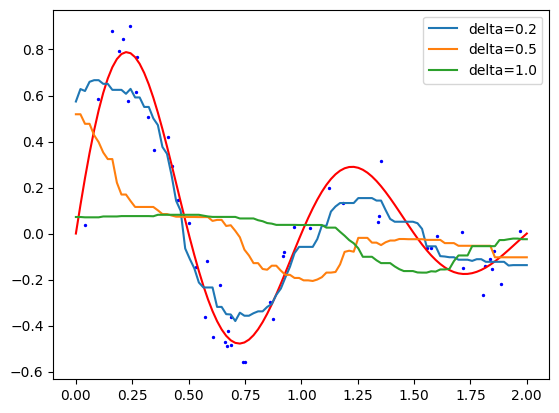
\includegraphics[scale=0.6]{img/kmeans_smoother.png}
      \caption{K means smoother} 
      \label{fig:kmeans_smoother}
    \end{figure}
  \end{example}

  \begin{code}[MWS of K Nearest Neighbor Regression in scikit-learn]
    Local averaging is implemented as the K nearest neighbor regressor in scikit learn. It is slightly different in the way that it doesn't use the points within a certain $\delta$ away but rather the $K$ nearest points. Either way, a minimal working example of this is 
    \begin{lstlisting}
      X = [[0], [1], [2], [3]]
      y = [0, 0, 1, 1]
      from sklearn.neighbors import KNeighborsRegressor
      neigh = KNeighborsRegressor(n_neighbors=2)
      neigh.fit(X, y)
      print(neigh.predict([[1.5]])) 
    \end{lstlisting}
  \end{code}

  Note that since $\hat{f}$ is a combination of step functions, this makes it discontinuous at points. 

